\documentclass[a4paper, 12pt]{article}

\usepackage[T2A]{fontenc}
\usepackage[utf8]{inputenc}
\usepackage[english,russian]{babel}

\usepackage{amsmath, amsfonts, amssymb, amsthm, mathtools}

\usepackage{pgfplots}
\pgfplotsset{compat=1.9}

\usepackage{graphicx}
\graphicspath{{pictures/}}
\DeclareGraphicsExtensions{.pdf,.png,.jpg}

\author{\textbf{Муляревич Андрей Игоревич}}
\title{
\begin{LARGE}
\textbf{Лабораторная работа 1.1.4}\\
"Измерение интенсивности космического излучения"
\end{LARGE}
}
\date{\today}

\begin{document}

\maketitle
\newpage
\textbf{Краткое описание и цель работы:} Измерение интенсивности космического излучения с помощью счетчика Гейгера-Мюллера. Длительность эксперимента 1 час 6 мин 40 сек. Для проведения эксперемента используется устоновка со счетчиком СГС-6, результаты работы которого обробатывает подключенный к нему компьютер. Счетчик СГС-6 представляет собой полый металлический циллиндр(катод) и металлическую нить(анод), проходящую вдоль оси циллинда. Полость заполнена газом. Когда заряженная частица проходит через газ, она вызывает его ионизацию, в итоге происходит пробой, информация о котором записывается в компьютере

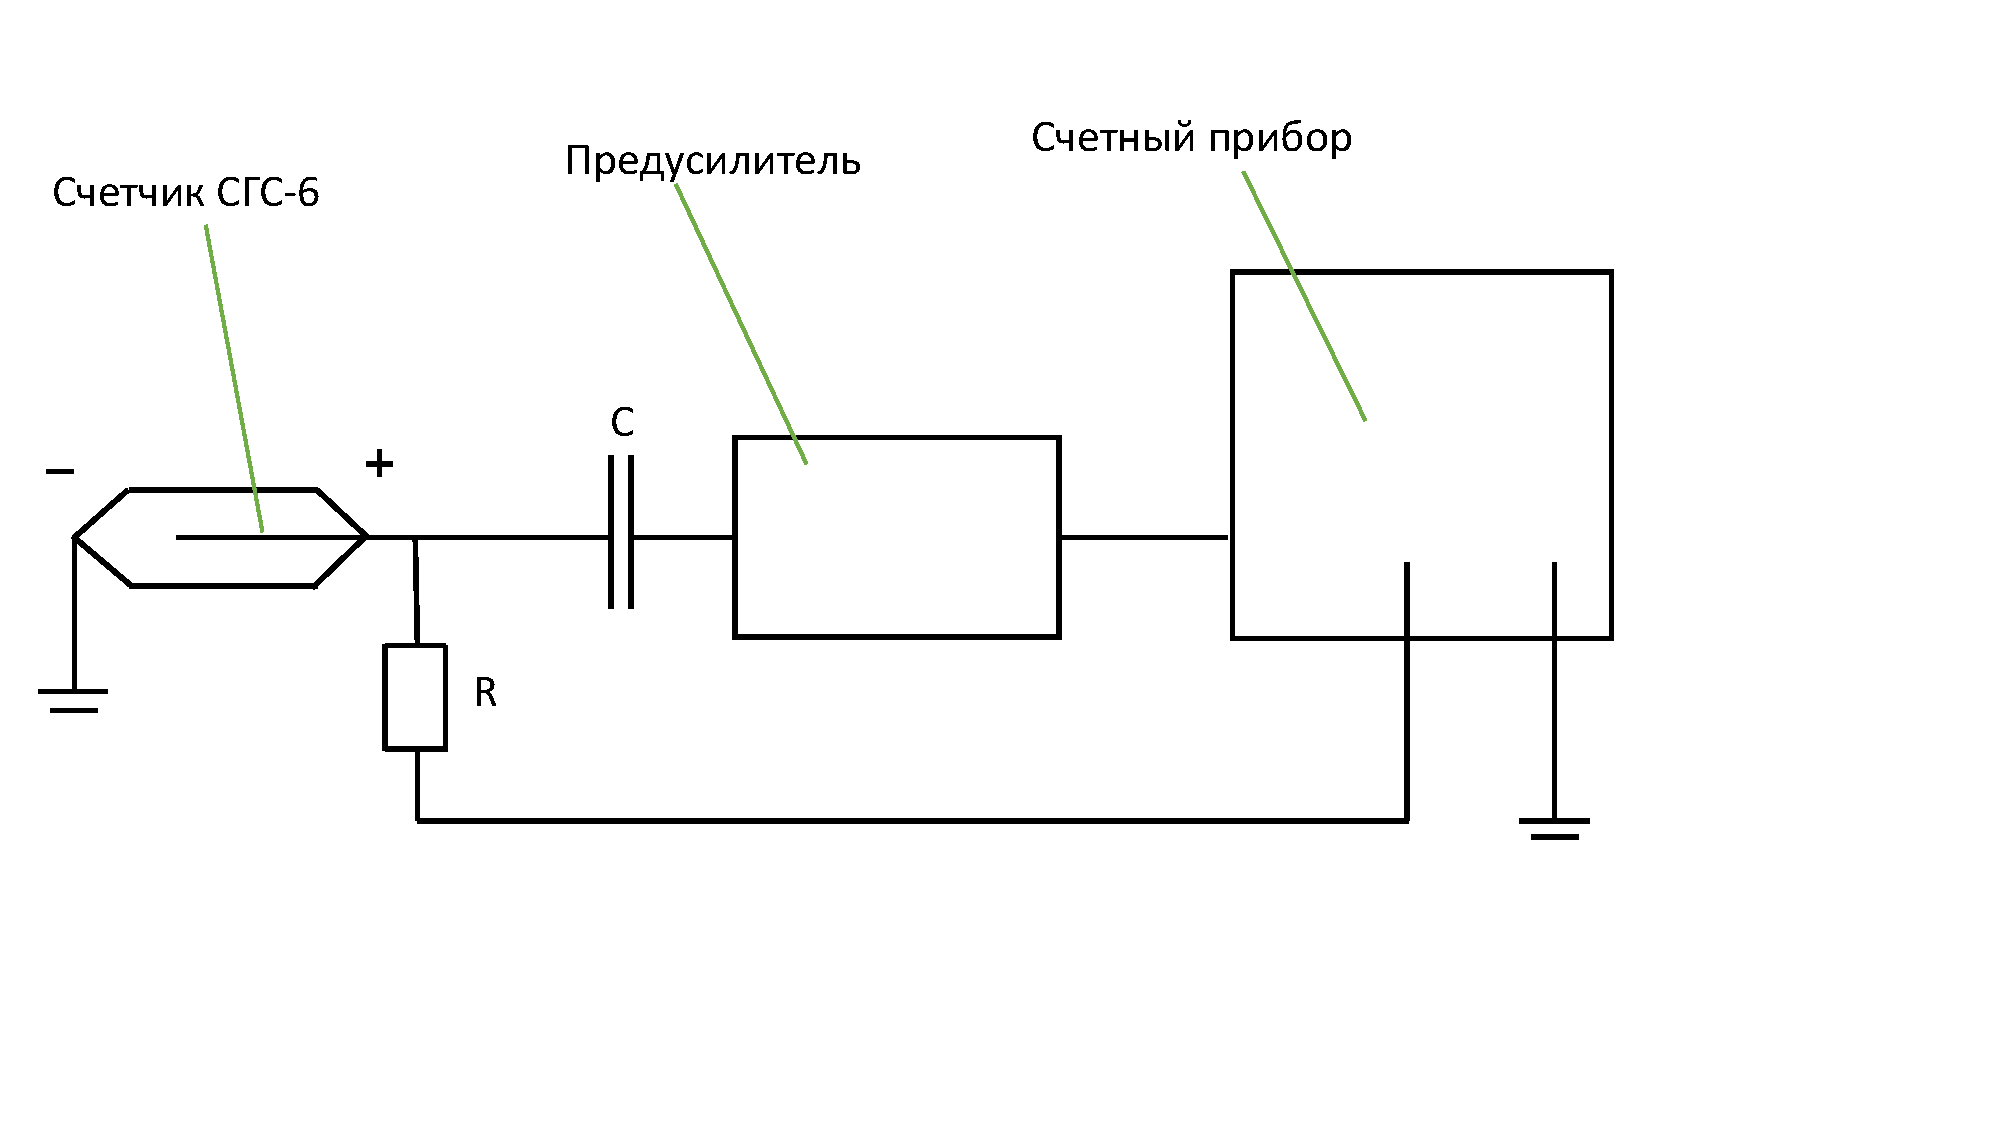
\includegraphics[scale=0.45]{shema.pdf} 

\textbf{Цель экспиремента}: применение методов обработки экспирементальных данных для изучения интенсивности излучения радиационного фона

\textbf{Порядок выполнения экспиремента:}
\begin{enumerate}
\item Включаем питание компьютера и установки. После загрузки компьютера запускаем программу STAT и таким образом начинаем проведение основного эксперимента. 
\item В результате демонстрационного эксперимента убеждаемся, что при увеличении числа измерений:
\begin{enumerate}
\item Измеряемая велечина флуктуирует;
\item Флуктуации среднего значения измеряемой величины уменьшаются, и среднее значение выходит на постоянную величину;
\item Флуктуации велечины погрешности среднего значения уменьшаются, а сама величина убывает;
\item Флуктуации величины погрешности отдельного измерения уменьшаются, и погрешность отдельного измерения (погрешность метода) выходит на постоянную величину.
\end{enumerate}
\item Переходим к основному эксперименту: измерение плотности потока космического излучения за 20 секунд (результаты набрались с момента включения компьютера). На компьютере проведем обработку, аналогичную сделанной в демонстрационном эксперименте. Результаты приведены в табл. 1.
\item Разбиваем результаты из табл. 1 в порядке их получения на группы по 2, что соответствует произведению $N_2 = 100$ измерений числа частиц за интервал времени, равный 40 с. Результаты приведем в табл. 2.
\item Приведем данные ддя построения гистограмм распределения числа срабатываний счетчика за 10 с и 40 с в таблицах табл. 3 и табл. 4 соответственно. 
\item Так же приведем гистограммы распределений среднего числа отсчетов за 10 и 40 с. (Рис. 1, 2) 
\item Используя формулы
\[ \overline{n}_1 = \dfrac{1}{N_1} \sum_{i = 1}^{N_1} {n_i} 
 \]
 \[ \overline{n}_2 = \dfrac{1}{N_2} \sum_{i = 1}^{N_2} {n_i} 
 \]
 \[ \overline{n}_3 = \dfrac{1}{N_3} \sum_{i = 1}^{N_3} {n_i} 
 \] 
\item Определим среднее число срабатываний счетчика за 10, 20 и 40 с соответственно.
\item Найдем среднеквадратичные ошибки \textbf{$\sigma$} отдельных измерений по формулам:
\[ \sigma_1 = \sqrt{\dfrac{1}{N_1 - 1} \sum_{i = 1}^{N_1} {(n_i - \overline{n}_1)^2} }
 \]
 \[ \sigma_2 = \sqrt{\dfrac{1}{N_2 - 1} \sum_{i = 1}^{N_2} {(n_i - \overline{n}_2)^2} }
 \]
 \[ \sigma_3 = \sqrt{\dfrac{1}{N_3 - 1} \sum_{i = 1}^{N_3} {(n_i - \overline{n}_3)^2} }
 \]
и убедимся в справедливости формул для примерного значения \textbf{$\sigma$}:
 \[\sigma_1^{'} \approx\sqrt{\overline{n}_1} \]
 \[\sigma_2^{'} \approx\sqrt{\overline{n}_2} \]
 \[\sigma_3^{'} \approx\sqrt{\overline{n}_3} \]
 \item найдем ошибки всех измерений \textbf{$\sigma^{''}$} по формулам
 \[ \sigma_1^{''} = \sqrt{\dfrac{1}{(N_1 - 1)N_1} \sum_{i = 1}^{N_1} {(n_i - \overline{n}_1)^2} }
 \]
 \[ \sigma_2^{''} = \sqrt{\dfrac{1}{(N_2 - 1)N_2} \sum_{i = 1}^{N_2} {(n_i - \overline{n}_2)^2} }
 \]
 \[ \sigma_3^{''} = \sqrt{\dfrac{1}{(N_3 - 1)N_3} \sum_{i = 1}^{N_3} {(n_i - \overline{n}_3)^2} }
 \]
\item Зафикисруем все полученные ошибки и среднии значения срабатываний в табл. 5.
\item Определим долю случаев, когда отклонения не превышают $\sigma_i$ и $2\sigma_i$, и сравним с теоретическими оценками (табл. 6).
\item Посчитаем относительную ошибку по формуле
\[ \varepsilon_{\overline{n}_1} = \dfrac{\sigma_{\overline{n}_1}}{\overline{n}_1} 100 \% \]
\[ \varepsilon_{\overline{n}_2} = \dfrac{\sigma_{\overline{n}_2}}{\overline{n}_2} 100 \% \]
\[ \varepsilon_{\overline{n}_3} = \dfrac{\sigma_{\overline{n}_3}}{\overline{n}_3} 100 \% \]
\item из табл. 6 следует, что $n_{t=10 c} = 12.46 \pm 0,18, \varepsilon_{\overline{n}_1} = 1,4 \%$, $n_{t=20 c} = 26,6 \pm 0,36, \varepsilon_{\overline{n}_2} = 1,4 \%$, $n_{t=40 c} = 53,11 \pm 0,61, \varepsilon_{\overline{n}_3} = 1,2 \%$
\end{enumerate}

\begin{tikzpicture}
\begin{axis}[
	height = 0.6\paperheight, 
	width = 0.6\paperwidth,
	ybar,
	title = Гистограмма Таблица 1,
	xlabel = {Число частиц за интервал 10 сек(Рис.1)},
	ylabel = {{\LARGE $\omega$}}
	]
\addplot coordinates
{ 
(3, 0.0025) (4, 0.005) (5, 0.0025) (6, 0.0275) (7, 0.03) (8, 0.045) (9, 0.1) (10, 0.0975) (11, 0.1125) (12, 0.115) (13, 0.0975) (14, 0.0825) (15, 0.0825) (16, 0.0525) (17, 0.06) (18, 0.035) (19, 0.0225) (20, 0.0175) (21, 0.0075) (22, 0.0025) (23, 0.0025)
};

\end{axis}
\end{tikzpicture}\\

\begin{tikzpicture}
\begin{axis}[
	height = 0.6\paperheight, 
	width = 0.6\paperwidth,
	ybar,
	title = Гистограмма Таблица 2,
	xlabel = {Число частиц за интервал 40 сек(Рис.2)},
	ylabel = {{\LARGE $\omega$}}
	]
\addplot[draw = red, bar width = 0.8] coordinates
{ 
(33, 0.01) (34, 0.02) (36, 0.01) (37, 0.01) (38, 0.01) (39, 0.01) (40, 0.02) (41, 0.03) (42, 0.02) (43, 0.04) (44, 0.07) (45, 0.05) (46, 0.04) (47, 0.04) (48, 0.08) (49, 0.06) (50, 0.05) (51, 0.05) (52, 0.06) (53, 0.06) (54, 0.03) (55, 0.04) (56 0.03) (57, 0.04) (58, 0.01) (59, 0.03) (60, 0.02) (62, 0.03) (63, 0.01) (64, 0.01) (66, 0.01) (67, 0.01) (69, 0.01)
};

\end{axis}
\end{tikzpicture}\\
\newpage
							%Таблица 1
\begin{table}
\caption{\textbf{Число срабатываний счетчика за 10 сек}}
\begin{tabular}{|c|c|c|c|c|c|c|c|c|c|c|}
\hline 
\textbf{№ опыта} & \textbf{1} & \textbf{2} & \textbf{3} & \textbf{4} & \textbf{5} & \textbf{6} & \textbf{7} & \textbf{8} & \textbf{9} & \textbf{10} \\ 
\hline 
\textbf{0}: & 30 & 26 & 23 & 25 & 28 & 31 & 28 & 20 & 29 & 30 \\ 
\hline 
\textbf{10}: & 27 & 17 & 23 & 21 & 23 & 20 & 26 & 27 & 21 & 26 \\ 
\hline 
\textbf{20}: & 27 & 30 & 22 & 27 & 31 & 23 & 22 & 28 & 24 & 24 \\ 
\hline 
\textbf{30}: & 22 & 29 & 25 & 25 & 26 & 26 & 18 & 30 & 32 & 31 \\ 
\hline\hline
\textbf{40}: & 35 & 22 & 32 & 20 & 26 & 12 & 22 & 22 & 20 & 21 \\ 
\hline 
\textbf{50}: & 18 & 26 & 20 & 21 & 27 & 25 & 21 & 24 & 30 & 28 \\ 
\hline 
\textbf{60}: & 33 & 31 & 25 & 20 & 22 & 21 & 19 & 18 & 25 & 27 \\ 
\hline 
\textbf{70}: & 16 & 18 & 28 & 24 & 24 & 24 & 21 & 19 & 24 & 25 \\ 
\hline\hline 
\textbf{80}: & 30 & 22 & 28 & 16 & 23 & 30 & 26 & 21 & 23 & 27 \\ 
\hline 
\textbf{90}: & 27 & 39 & 26 & 19 & 26 & 25 & 25 & 22 & 22 & 21 \\ 
\hline 
\textbf{100}: & 34 & 26 & 20 & 31 & 18 & 28 & 20 & 25 & 27 & 28 \\ 
\hline 
\textbf{110}: & 32 & 21 & 15 & 34 & 23 & 27 & 25 & 30 & 30 & 25\\
\hline\hline
\textbf{120}: & 22 & 22 & 22 & 24 & 15 & 27 & 22 & 32 & 30 & 32 \\ 
\hline 
\textbf{130}: & 30 & 16 & 23 & 25 & 19 & 23 & 31 & 26 & 24 & 29 \\ 
\hline 
\textbf{140}: & 22 & 27 & 18 & 27 & 41 & 28 & 17 & 22 & 30 & 25 \\ 
\hline 
\textbf{150}: & 19 & 29 & 28 & 23 & 27 & 26 & 15 & 19 & 26 & 31 \\ 
\hline\hline
\textbf{160}: & 33 & 29 & 23 & 13 & 26 & 25 & 31 & 22 & 27 & 20 \\ 
\hline 
\textbf{170}: & 22 & 32 & 36 & 31 & 15 & 18 & 22 & 27 & 25 & 25 \\ 
\hline 
\textbf{180}: & 18 & 21 & 29 & 27 & 28 & 28 & 31 & 31 & 24 & 24 \\ 
\hline 
\textbf{190}: & 19 & 23 & 29 & 30 & 22 & 22 & 22 & 27 & 35 & 25 \\ 
\hline 
\end{tabular}
\end{table}
						%Таблица 2
\begin{table}
\caption{\textbf{Число срабатываний счетчика за 40 сек}}
\begin{tabular}{|c|c|c|c|c|c|c|c|c|c|c|}
\hline 
\textbf{№ опыта} & \textbf{1} & \textbf{2} & \textbf{3} & \textbf{4} & \textbf{5} & \textbf{6} & \textbf{7} & \textbf{8} & \textbf{9} & \textbf{10} \\ 
\hline 
\textbf{0} & 56 & 48 & 59 & 48 & 59 & 43 & 44 & 43 & 53 & 47 \\ 
\hline 
\textbf{10} & 57 & 49 & 54 & 50 & 48 & 51 & 50 & 52 & 48 & 63 \\ 
\hline\hline 
\textbf{20} & 57 & 52 & 38 & 44 & 41 & 44 & 41 & 52 & 45 & 58 \\ 
\hline 
\textbf{30} & 64 & 45 & 43 & 37 & 52 & 34 & 52 & 48 & 40 & 49 \\ 
\hline\hline
\textbf{40} & 52 & 44 & 53 & 47 & 50 & 66 & 45 & 51 & 47 & 43 \\ 
\hline 
\textbf{50} & 60 & 51 & 46 & 45 & 55 & 53 & 49 & 50 & 55 & 55 \\ 
\hline\hline 
\textbf{60} & 44 & 46 & 42 & 54 & 62 & 46 & 48 & 42 & 57 & 53 \\ 
\hline 
\textbf{70} & 49 & 45 & 69 & 39 & 55 & 48 & 51 & 53 & 34 & 57 \\ 
\hline\hline 
\textbf{80} & 62 & 36 & 51 & 53 & 47 & 54 & 67 & 33 & 49 & 50 \\ 
\hline 
\textbf{90} & 39 & 56 & 56 & 62 & 48 & 41 & 59 & 44 & 49 & 60 \\ 
\hline 
\end{tabular} 
\end{table}
								%Таблица 3
\begin{table}
\caption{\textbf{Данные для построения гистограммы распределения числа срабатываний счетчиков за 10 с}}
\begin{tabular}{|c|c|c|}
\hline 
\textbf{Число импульсов} & \textbf{Число случаев} & \textbf{Доля случаев} \\ 
\hline 
3 & 1 & 0,0025 \\ 
\hline 
4 & 2 & 0,005 \\ 
\hline 
5 & 1 & 0,0025 \\ 
\hline 
6 & 11 & 0,0275 \\ 
\hline 
7 & 12 & 0,03 \\ 
\hline 
8 & 18 & 0,045 \\ 
\hline 
9 & 40 & 0,1 \\ 
\hline 
10 & 39 & 0,0975 \\ 
\hline 
11 & 45 & 0,1125 \\ 
\hline 
12 & 46 & 0,115 \\ 
\hline 
13 & 39 & 0,0975 \\ 
\hline 
14 & 33 & 0,0825 \\ 
\hline 
15 & 33 & 0,0825 \\ 
\hline 
16 & 21 & 0,0525 \\ 
\hline 
17 & 24 & 0,06 \\ 
\hline 
18 & 14 & 0,035 \\ 
\hline 
19 & 9 & 0,0225 \\ 
\hline 
20 & 7 & 0,0175 \\ 
\hline 
21 & 3 & 0,0075 \\ 
\hline 
22 & 1 & 0,0025 \\
\hline  
23 & 1 & 0,0025 \\ 
\hline 
\end{tabular} 
\end{table}
\newpage
								%Таблица 4
\begin{table}
\caption{\textbf{ Данные для построения гистограммы распределения числа срабатываний счетчиков за 40 сек}}
\begin{tabular}{|c|c|c|}
\hline 
Число импульсов & Число случаев & Доля случаев \\ 
\hline 
33 & 1 & 0.01 \\ 
\hline 
34 & 2 & 0.02 \\ 
\hline
36 & 1 & 0.01 \\
\hline 
37 & 1 & 0.01 \\ 
\hline 
38 & 1 & 0.01 \\ 
\hline 
39 & 1 & 0.01 \\ 
\hline 
40 & 2 & 0.02 \\ 
\hline 
41 & 3 & 0.03 \\ 
\hline 
42 & 2 & 0.02 \\ 
\hline 
43 & 4 & 0.04 \\ 
\hline 
44 & 7 & 0.07 \\ 
\hline 
45 & 5 & 0.05 \\ 
\hline 
46 & 4 & 0.04 \\ 
\hline 
47 & 4 & 0.04 \\ 
\hline 
48 & 8 & 0.08 \\ 
\hline 
49 & 6 & 0.06 \\ 
\hline 
50 & 5 & 0.05 \\ 
\hline 
51 & 5 & 0.05 \\ 
\hline 
52 & 6 & 0.06 \\ 
\hline 
53 & 6 & 0.06 \\ 
\hline 
54 & 3 & 0.03 \\ 
\hline 
55 & 4 & 0.04 \\ 
\hline 
56 & 3 & 0.03 \\ 
\hline 
57 & 4 & 0.04 \\ 
\hline 
58 & 1 & 0.01 \\ 
\hline 
59 & 3 & 0.03 \\ 
\hline 
60 & 2 & 0.02 \\  
\hline 
62 & 3 & 0.03 \\ 
\hline 
63 & 1 & 0.01 \\ 
\hline 
64 & 1 & 0.01 \\ 
\hline 
66 & 1 & 0.01 \\ 
\hline 
67 & 1 & 0.01 \\ 
\hline  
69 & 1 & 0.01 \\ 
\hline 
\end{tabular}
\end{table}
\newpage
\begin{table}
\caption{\textbf{Ошибки и средние значения}}
\begin{tabular}{|c|c|c|c|c|c|}
\hline
&$\overline{n}$&$\sigma$&$\sigma^{'}$&$\sigma^{''}$&$\varepsilon_{\overline{n}}$\\
\hline
1&12.47&3.54&3.53&0,18&1.40 \\
\hline
2&24.93&5.10&5.00&0,35&1.42\\
\hline
3&49.86&6.89&7.06&0,61&1.38 \\
\hline
\end{tabular}
\caption{\textbf{Процент попадания точек в промежуток среднего значения с учетом погрешности}}
\begin{tabular}{|c|c|c|c|c|}
\hline
Значение&Ошибка&Число случаев&Доля случаев,$\%$&Теоретическая оценка,$\%$ \\
\hline
$\overline{n}_1 = 12.465$ & $\pm \sigma_1 = \pm 3.54$ & 286 & 71 & 68 \\
& $\pm 2 \sigma_1 = \pm 7.08$ & 389 & 97 & 95 \\
\hline
$\overline{n}_2 = 24.93$ & $\pm  \sigma_2 = \pm 5.10$ & 138 & 69 & 68 \\
& $\pm 2 \sigma_2 = \pm 10.20$ & 192 & 96 & 95 \\
\hline
$\overline{n}_3 = 49.86$ & $\pm  \sigma_3 = \pm 6.89$ & 68 & 68 & 68 \\
& $\pm 2 \sigma_3 = \pm 13.78$ & 96 & 96 & 95 \\
\hline
\end{tabular}
\end{table}

\end{document}